% Draft for \subsection{Agent Trajectory Compaction} of IB/evaluation_section_snapshot.tex. Updated Oct 14 ~14:10Z to the
% H0 pair's figure (arm A + 608 more training runs; chosen on development numbers by the rule fixed in advance). Every number
% below is from IB/ARTIFACTS/PAPER_COMPACTION/figs/frozen100_h0_fig.json and the paired analysis in RESULTS_SO_FAR.md.
% Not merged into the snapshot. A 9B-written-prefix version of the benchmark is running and may replace the setup.
%
% Sentences of the current snapshot this figure refutes or does not support (to drop or rewrite):
%   - "even matching/exceeding an untuned model with full context": not exceeding; at 1/5 and 1/10 AC rows finish at the
%     full prefix's cost but solve 8 fewer (paired -8 [-16, +1]; not significant).
%   - "a 1/10th compression, it is effectively as good as seeing the whole context": on cost to finish, yes (12.3k vs 11.3k
%     tokens, not significant); on solved, 47 vs 55 (not significant, interval touches 0). Defensible only with that caveat.
%   - "beats truncation and summarization": truncation, yes (solved at 1/10 and 1/20, tokens at every size); summary, ties on
%     solved at 1/5 and 1/10 (+2) and beats it on tokens (-6.4k to -7.5k) and time.
%   - "an order of magnitude faster": no; 1.3 s against 7.4 s, about 5.5x, one run per GPU.
%   - "Improvements are even better when vectors are combined with truncation": not run (AC + recent text is not in the MVP).
%   - The setup paragraphs also differ from what ran: Java, Python and Kotlin (not Java only); prefixes cut at 20k inside
%     20k--50k runs (not 32k); continuation budget 30k; 100 evaluation prefixes (not 200); ratios 1/5, 1/10, 1/20 (not 1/4
%     ... 1/32); shared prefix written by the 27B; training targets are the untuned 9B's own full-context continuations; no
%     unrelated-task training data in this run.

\textbf{Datasets and Benchmarks}
We consider long-horizon tasks from Long Code Arena (LCA) Bug Localization (Java, Python and Kotlin), split by
repository into training and evaluation sides. A Qwen 3.8 27B agent at medium reasoning first runs a large pool of
tasks. Runs that end between 20k and 50k tokens are cut at the first tool result past 20k tokens; that prefix is
shared by every variant, and the agent must resume from it. We evaluate on 100 such prefixes from evaluation-side
repositories (46 Python, 36 Java, 18 Kotlin; mean prefix 19.7k tokens) with a continuation budget of 30k tokens; an
unanswered run counts the whole budget. Training uses only training-side repositories: the untuned 9B resumes
training prefixes with the full prefix in view, and the continuations that solve their task are the targets.

\textbf{Comparisons}
The resuming agent is always Qwen 3.5 9B (thinking on). It sees the full prefix, nothing, the most recent text
truncated to 1/5, 1/10 or 1/20 of the prefix, or a summary it wrote itself when asked to compact (the summarization
used in most harnesses). The AC variant replaces the prefix by 4,000, 2,000 or 1,000 AC rows produced by Qwen 3.5
2B with adapter modules; the 9B reader carries a LoRA adapter trained jointly with the encoder.

\textbf{Training}
The encoder (Qwen 3.5 2B with adapter modules) and a LoRA adapter on the 9B reader start from a pair trained to reconstruct
long contexts from 1/10 of their length. They are then trained jointly to continue agent runs: for 908 solved training
runs, the target is the untuned 9B's own continuation of the 27B prefix with the full prefix in view, and the prefix is
replaced by AC rows at 8 sizes drawn log-uniformly between 1/20 and 1/5 of its length (cross-entropy, learning rate
$2\times10^{-5}$ for both, one pass). The pair is selected on 50 separate development prefixes, never on the evaluation prefixes.

\textbf{Results}
\begin{figure}[t]
  \centering
  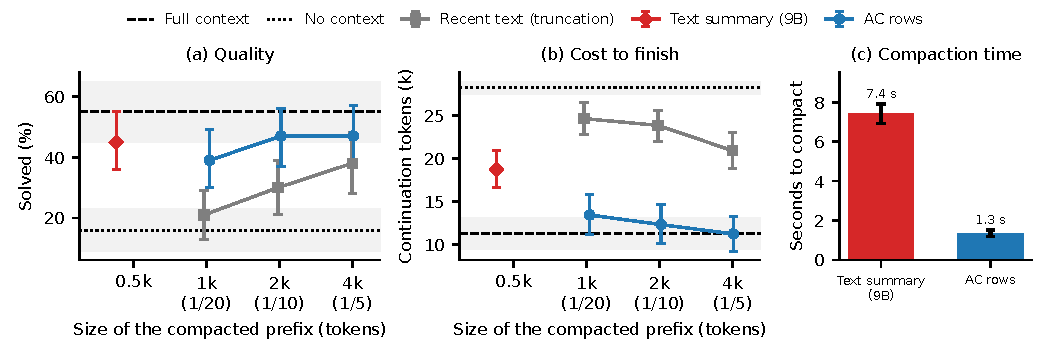
\includegraphics[width=\linewidth]{figs/frozen100_h0_fig.pdf}
  \caption{Resuming 100 Long Code Arena bug-localization runs from a shared 27B-written prefix (mean 19.7k tokens).
  (a) Share of tasks solved, (b) continuation tokens to finish (unanswered runs count the 30k budget), against the
  size of what replaces the prefix. (c) Seconds to produce the compaction, one run per GPU. Error bars and bands:
  95\% bootstrap intervals over prefixes.}
  \label{fig:evalCompaction}
\end{figure}
The compaction results are shown in \cref{fig:evalCompaction}. With AC rows the agent picks up where the prefix left off:
at 1/5 and 1/10 it answers 88 and 82 of 100 tasks and needs 11.3k and 12.3k continuation tokens, the same cost as with
the full prefix (91 answered, 11.3k tokens; paired differences not significant). With truncated text of the same size it
answers 55 and 44 and needs 20.9k and 23.9k tokens, and with its own summary it answers 67 and needs 18.8k. AC rows need
9.7k to 11.5k fewer tokens than truncation at every size, and 5.3k to 7.5k fewer than the summary.

On the share of tasks solved, AC rows solve 47, 47 and 39 tasks at 1/5, 1/10 and 1/20, against 38, 30 and 21 for
truncation (paired $+17$ and $+18$ at 1/10 and 1/20, $p<0.01$) and 45 for the 9B's own summary, which they match at
1/5 and 1/10. The full prefix solves 55; the gap of 8 at 1/5 and 1/10 is within the noise of 100 prefixes.

We also compare the time taken to produce a text compaction and a vector compaction (\cref{fig:evalCompaction}c,
one run at a time on an RTX PRO 6000 Blackwell GPU). Writing the summary is a 510-token decode by the 9B that takes
7.4\,s; the AC rows are one encoder pass of the 2B model over the prefix and take 1.3\,s, about 5.5 times faster.
Truncation needs no model call at all, but it is also the variant that leaves the agent the most work to redo.

We conclude from this section that AC rows at a tenth of the prefix let an agent resume a long trajectory at the cost of
the full context and solve as many tasks as with a text summary, while being several times cheaper to produce than that
summary.
